\documentclass{article}
\usepackage[margin=1in]{geometry}
\usepackage{titlesec}
\usepackage[table]{xcolor}
\usepackage{float}
\usepackage{graphicx}
\graphicspath{{./}}

\titlelabel{\thetitle.\quad}
\definecolor{Gray}{gray}{0.9}

\title{\textbf{Time-Series Prediction using Multilayer Perceptron}}
\author{
    \textbf{Joseph Nguyen} \\
    \textit{Department of Computer Science} \\
    \textit{Franklin \& Marshall College} \\
    \textit{jnguyen2@fandm.edu}
}
\date{}

\begin{document}
\maketitle
\begin{abstract}
    This paper explores the effectiveness of the Multilayer Perceptron (MLP) class of neural networks in solving time-series prediction problems. The example problem in this paper is the prediction of ground-level ozone concentration in Harris County, Texas over time. The problem is formulated as a regression problem through the "rolling window" technique. This formulation makes the problem tractable for MLP neural networks. The results of experimentation show that MLP is most effective at predicting when the time interval between samples are small. Increasing the time interval between samples results in a significant drop in predictive performance. This paper makes contributions to research on effective approaches to time-series prediction problems and the limits of application for MLP neural networks.
\end{abstract}

\section{Introduction}
Ozone pollution is a serious issue that negatively affects the air quality and health of residents in large urban areas. In the atmosphere, ozone is good as it protects us from solar UV radiation. However, when it is on the ground, it can damage respiratory tissue and make it harder to breathe. The 2015 National Ambient Air Quality Standards (NAAQS) for ozone established by the EPA require that ambient air contains an ozone concentration of less than 0.07 ppm. \cite{epanaaqs}

In this paper, we will apply Multilayer Perceptron (MLP), a fundamental class of neural networks, to tackle the problem of time-series prediction of ozone concentration. The ability to predict the ozone concentration in the air is important because cities need to be able to determine when they should call for Ozone Action Days. This preventive measure is necessary for groups sensitive to air conditions such as children, older adults, and adults with asthma or lung disease. Beyond the problem-specific benefits, this paper will also shed light on whether MLP is an effective approach to time-series prediction problems.

\section{Approach}
In class, we have observed that a time-series prediction problem can be formulated as a regression problem. To formulate a time-series prediction problem as a regression problem and construct a training dataset for supervised learning methods, samples were generated using the rolling window method. \cite{rollingwindow} That is, in order to train a model to predict the value at an arbitrary time, t, the inputs are the values for that variable at ($t - 1$), ($t - 2$) ... ($t - n$), where $n$ is the size of the rolling window. There was also a bias feature added to each sample.

Real world data values can vary widely. We believe that MLP is more suited to handle this task than traditional linear regression methods. For instance, there are many parameters that can be tweaked in order to achieve optimal predictive performance with MLP. This flexibility allows MLP to learn complex non-linear relationships. 

The dataset used was directly obtained from the website of the United States Environmental Protection Agency. It contains 34,180 hourly samples from an air quality measurement station in Houston, Texas from January 1, 2012, to January 1, 2016. The values for ozone concentration in the dataset range from 0.000 ppm to 0.111 ppm. Figure 1 contains a visualization of the data. The dotted red line indicates the concentration level at which ozone becomes dangerous for humans exposed to it for 8 hours doing light work \cite{oshalimits} and the dotted yellow line indicates the NAAQS for ozone.

\begin{figure}[H]
    \begin{center}
        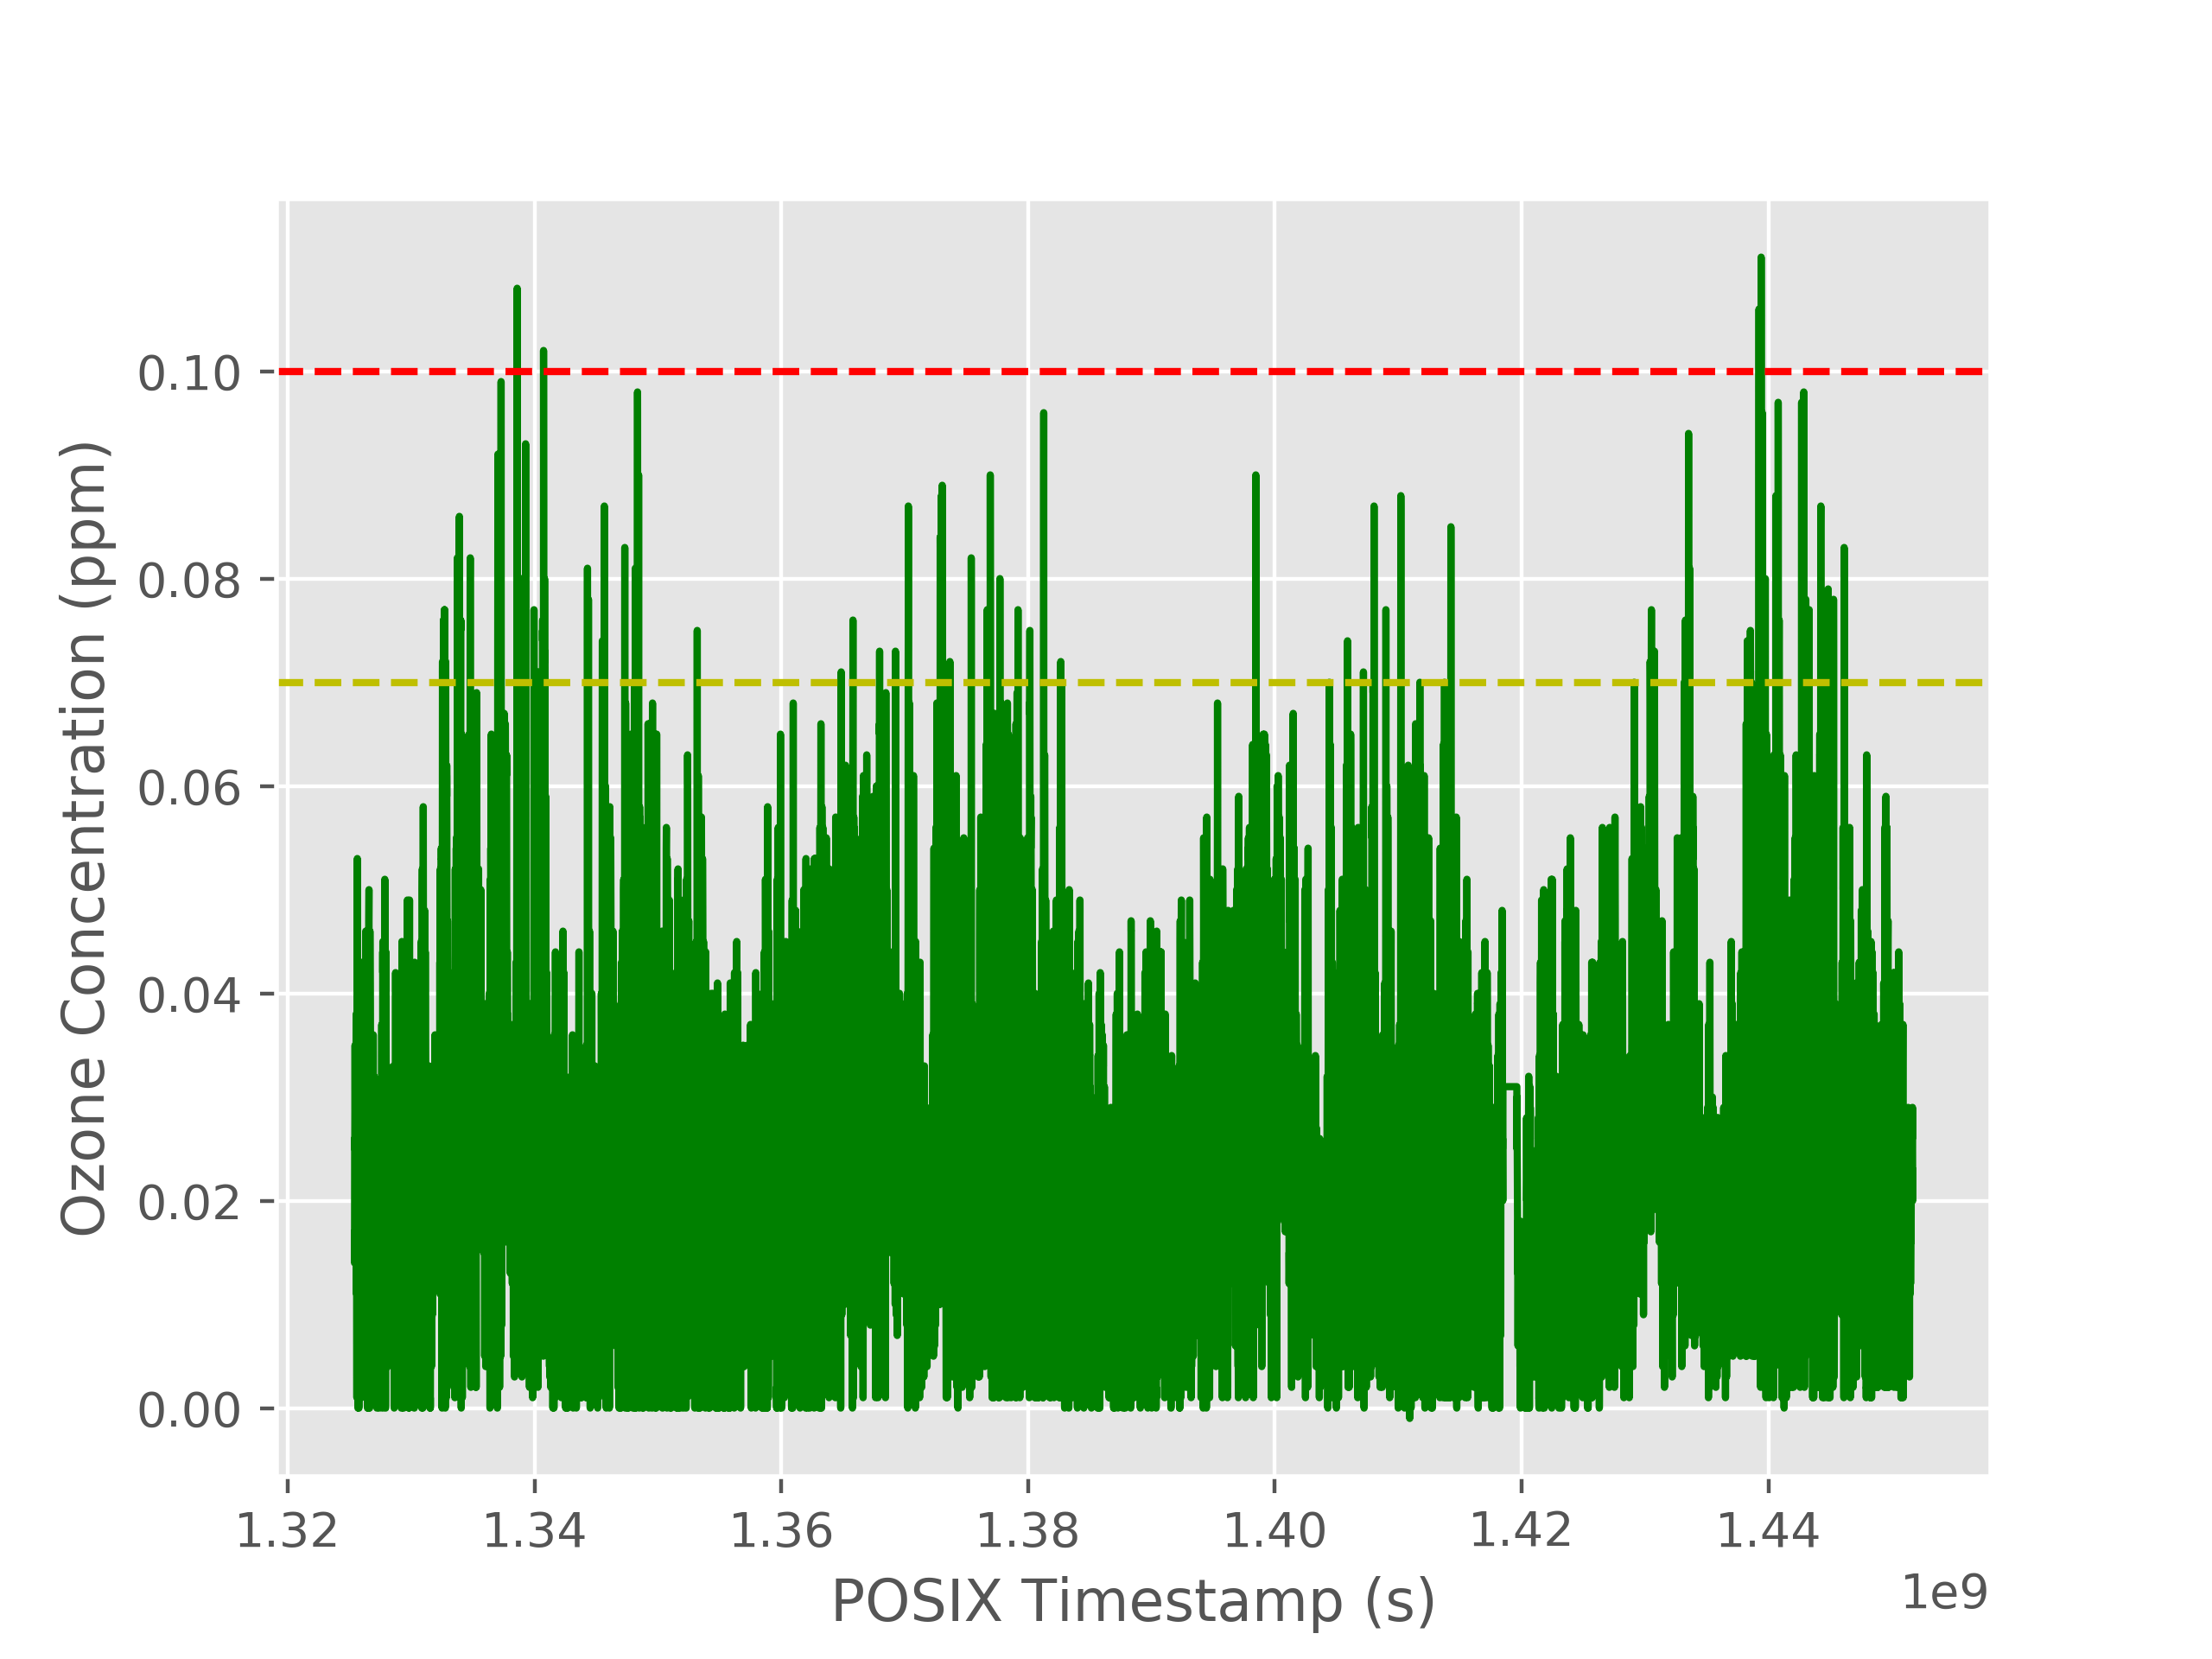
\includegraphics[scale=0.75]{ALLDATA.png}
    \end{center}
    \caption{Ozone concentration in parts per million from January 1, 2012 to January 1, 2016 in Harris County, Texas.}
\end{figure}

The data was preprocessed for this project. The formatted timestamps in the original dataset were converted to POSIX timestamps for easy computational interpretation and sorting. Missing data points were replaced with the most recently encountered actual value. Duplicate timestamps were removed from the dataset.  Data values were normalized in order to mitigate MLP sensitivity to scale.

\section{Experimentation}
The coefficient of determination, $r^2$, was the performance measure of choice as it is commonly used to evaluate regression models. The value of $r^2$ ranges from 0 to 1. A value close to zero indicates that the model is a poor fit. A value close to one indicates that the model is a near perfect fit. Some computational models can report a negative $r^2$ value. This is dependent on the definition of $r^2$ used and usually indicates the model may fit reasonably well but need some adjustments to the intercept.

The parameters for an MLP neural network can have a significant impact on its performance. As such, many different networks were constructed with different combinations of activation functions and amounts of hidden nodes and tested. Each network combination was tested in 10 trials in an attempt to reduce the noise for evaluation. Over these 10 trials, the $r^2$ value was summed and averaged. To ensure that the MLP learned the general relationship between data values at previous timestamps instead of the general trend over time, the training samples were shuffled before training in every trial. Due to the size of the dataset, cross-validation is not necessary. There was, however, a test set that was used to evaluate the performance of the MLP. This test set was composed of a randomized 20\% of the training data.

The neural networks were also trained and evaluated on their predictive ability for small and large time intervals. For instance, we tried to test the predictive performance of the MLP using hourly samples and daily samples. For the hourly samples, the data did not require any transformation other than picking the size of the rolling window. For the daily samples, the data was transformed by only picking out the values that occurred in 24-hour intervals.

\section{Results}

Below are the results from the experimentation procedures executed above.

\begin{figure}[H]
    \centering
    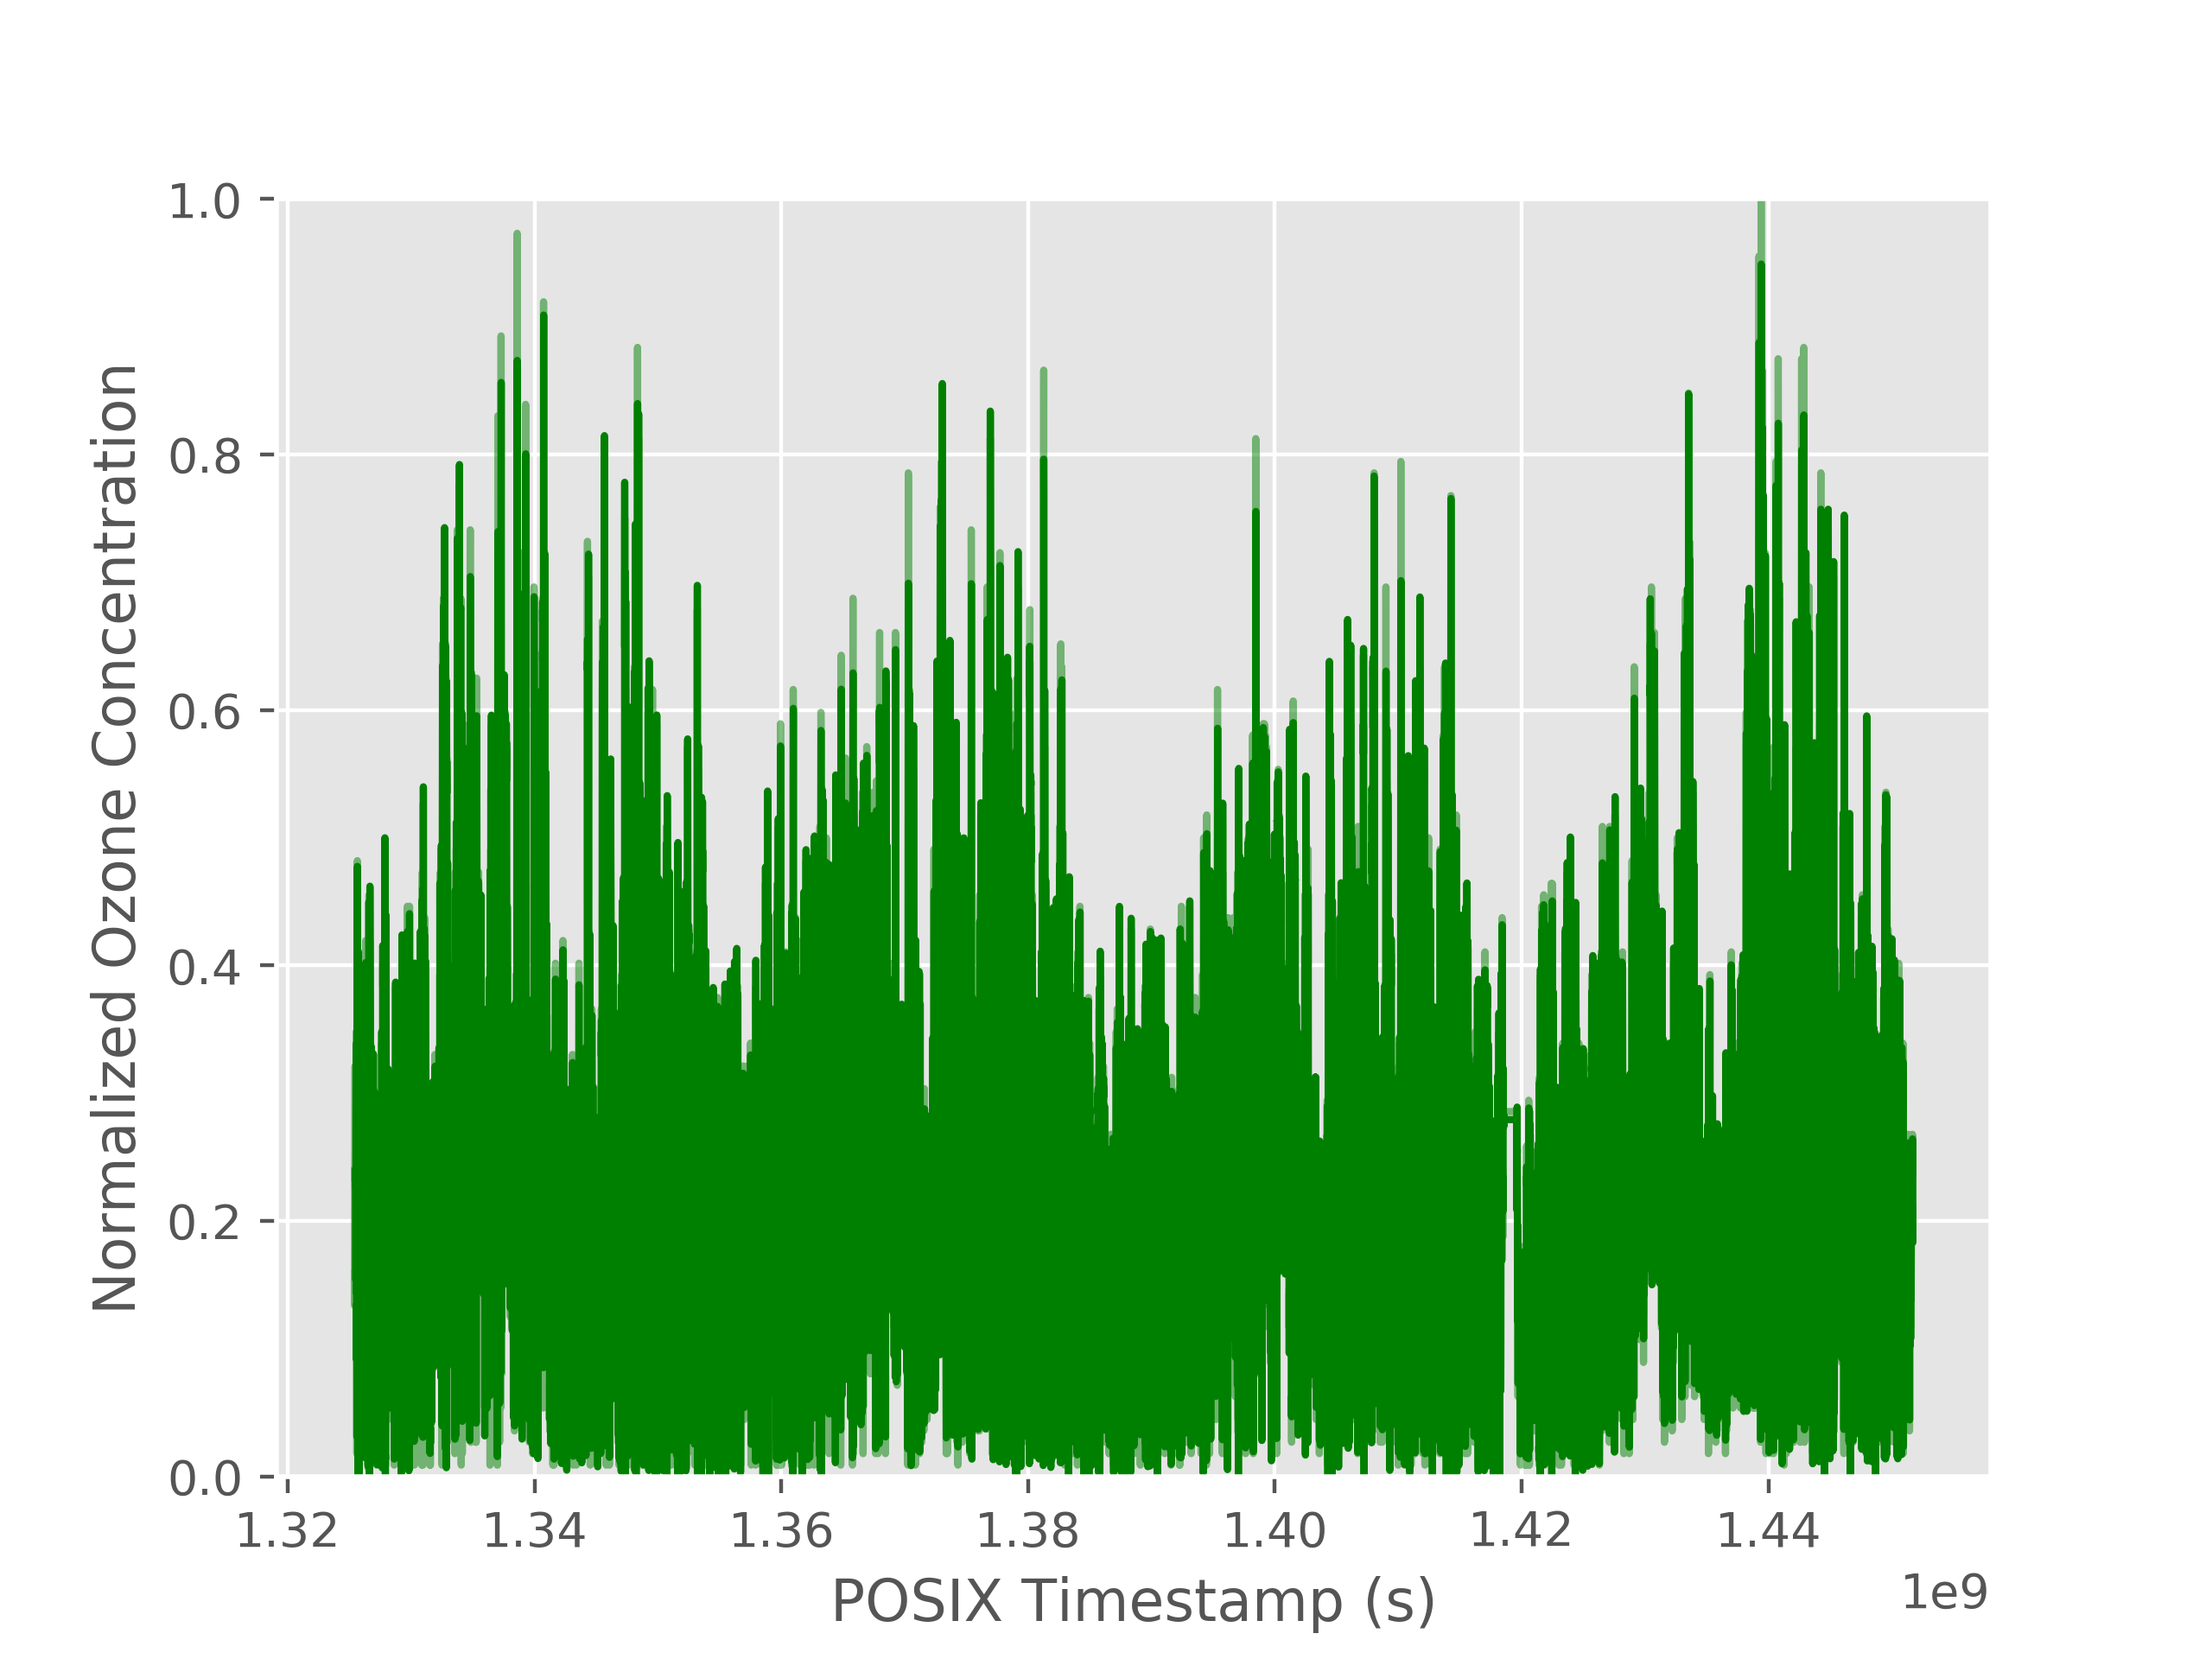
\includegraphics[scale=0.65]{H25_1500_RELU.png}
    \caption{Graph of actual data values and the best prediction for MLP trained using hourly data with a rolling window size of 25.}
\end{figure}

\begin{table}[H]
    \centering
    \begin{tabular}{| c | c | c | c | c |}
        \hline
        \cellcolor{black} & \cellcolor{Gray} 500 & \cellcolor{Gray} 1000 & \cellcolor{Gray} 1500 & \cellcolor{Gray} 2000 \\
        \hline
        \cellcolor{Gray} Identity & 0.9404 & 0.9409 & 0.9419 & 0.9392 \\
        \hline
        \cellcolor{Gray} Logistic & 0.9404 & 0.9391 & 0.9387 & 0.9359 \\
        \hline
        \cellcolor{Gray} Tanh & 0.9417 & 0.9408 & 0.9408 & 0.9400 \\
        \hline
        \cellcolor{Gray} ReLU & 0.9447 & 0.9432 & \cellcolor{green} 0.9452 & 0.9451 \\
        \hline
    \end{tabular}
    \caption{$r^2$ values for the time-series predictions of neural networks with different hidden layer activation functions and varying numbers of hidden nodes.}
\end{table}

Hourly prediction using MLP is pretty effective. In figure 2, the predictions accurately follow the trends of the data and the predictions are very close. Table 1 shows that the best performing MLP achieves an $r^2$ of 0.9452. The best performance is achieved with 1000 hidden nodes and the \textit{relu} activation function, however, the changing of these parameters did not seem to have a substantial impact on the predictive performance as initially expected, especially not as the MLP can learn the trend between data at past hours with relative ease.

\begin{figure}[H]
    \begin{center}
        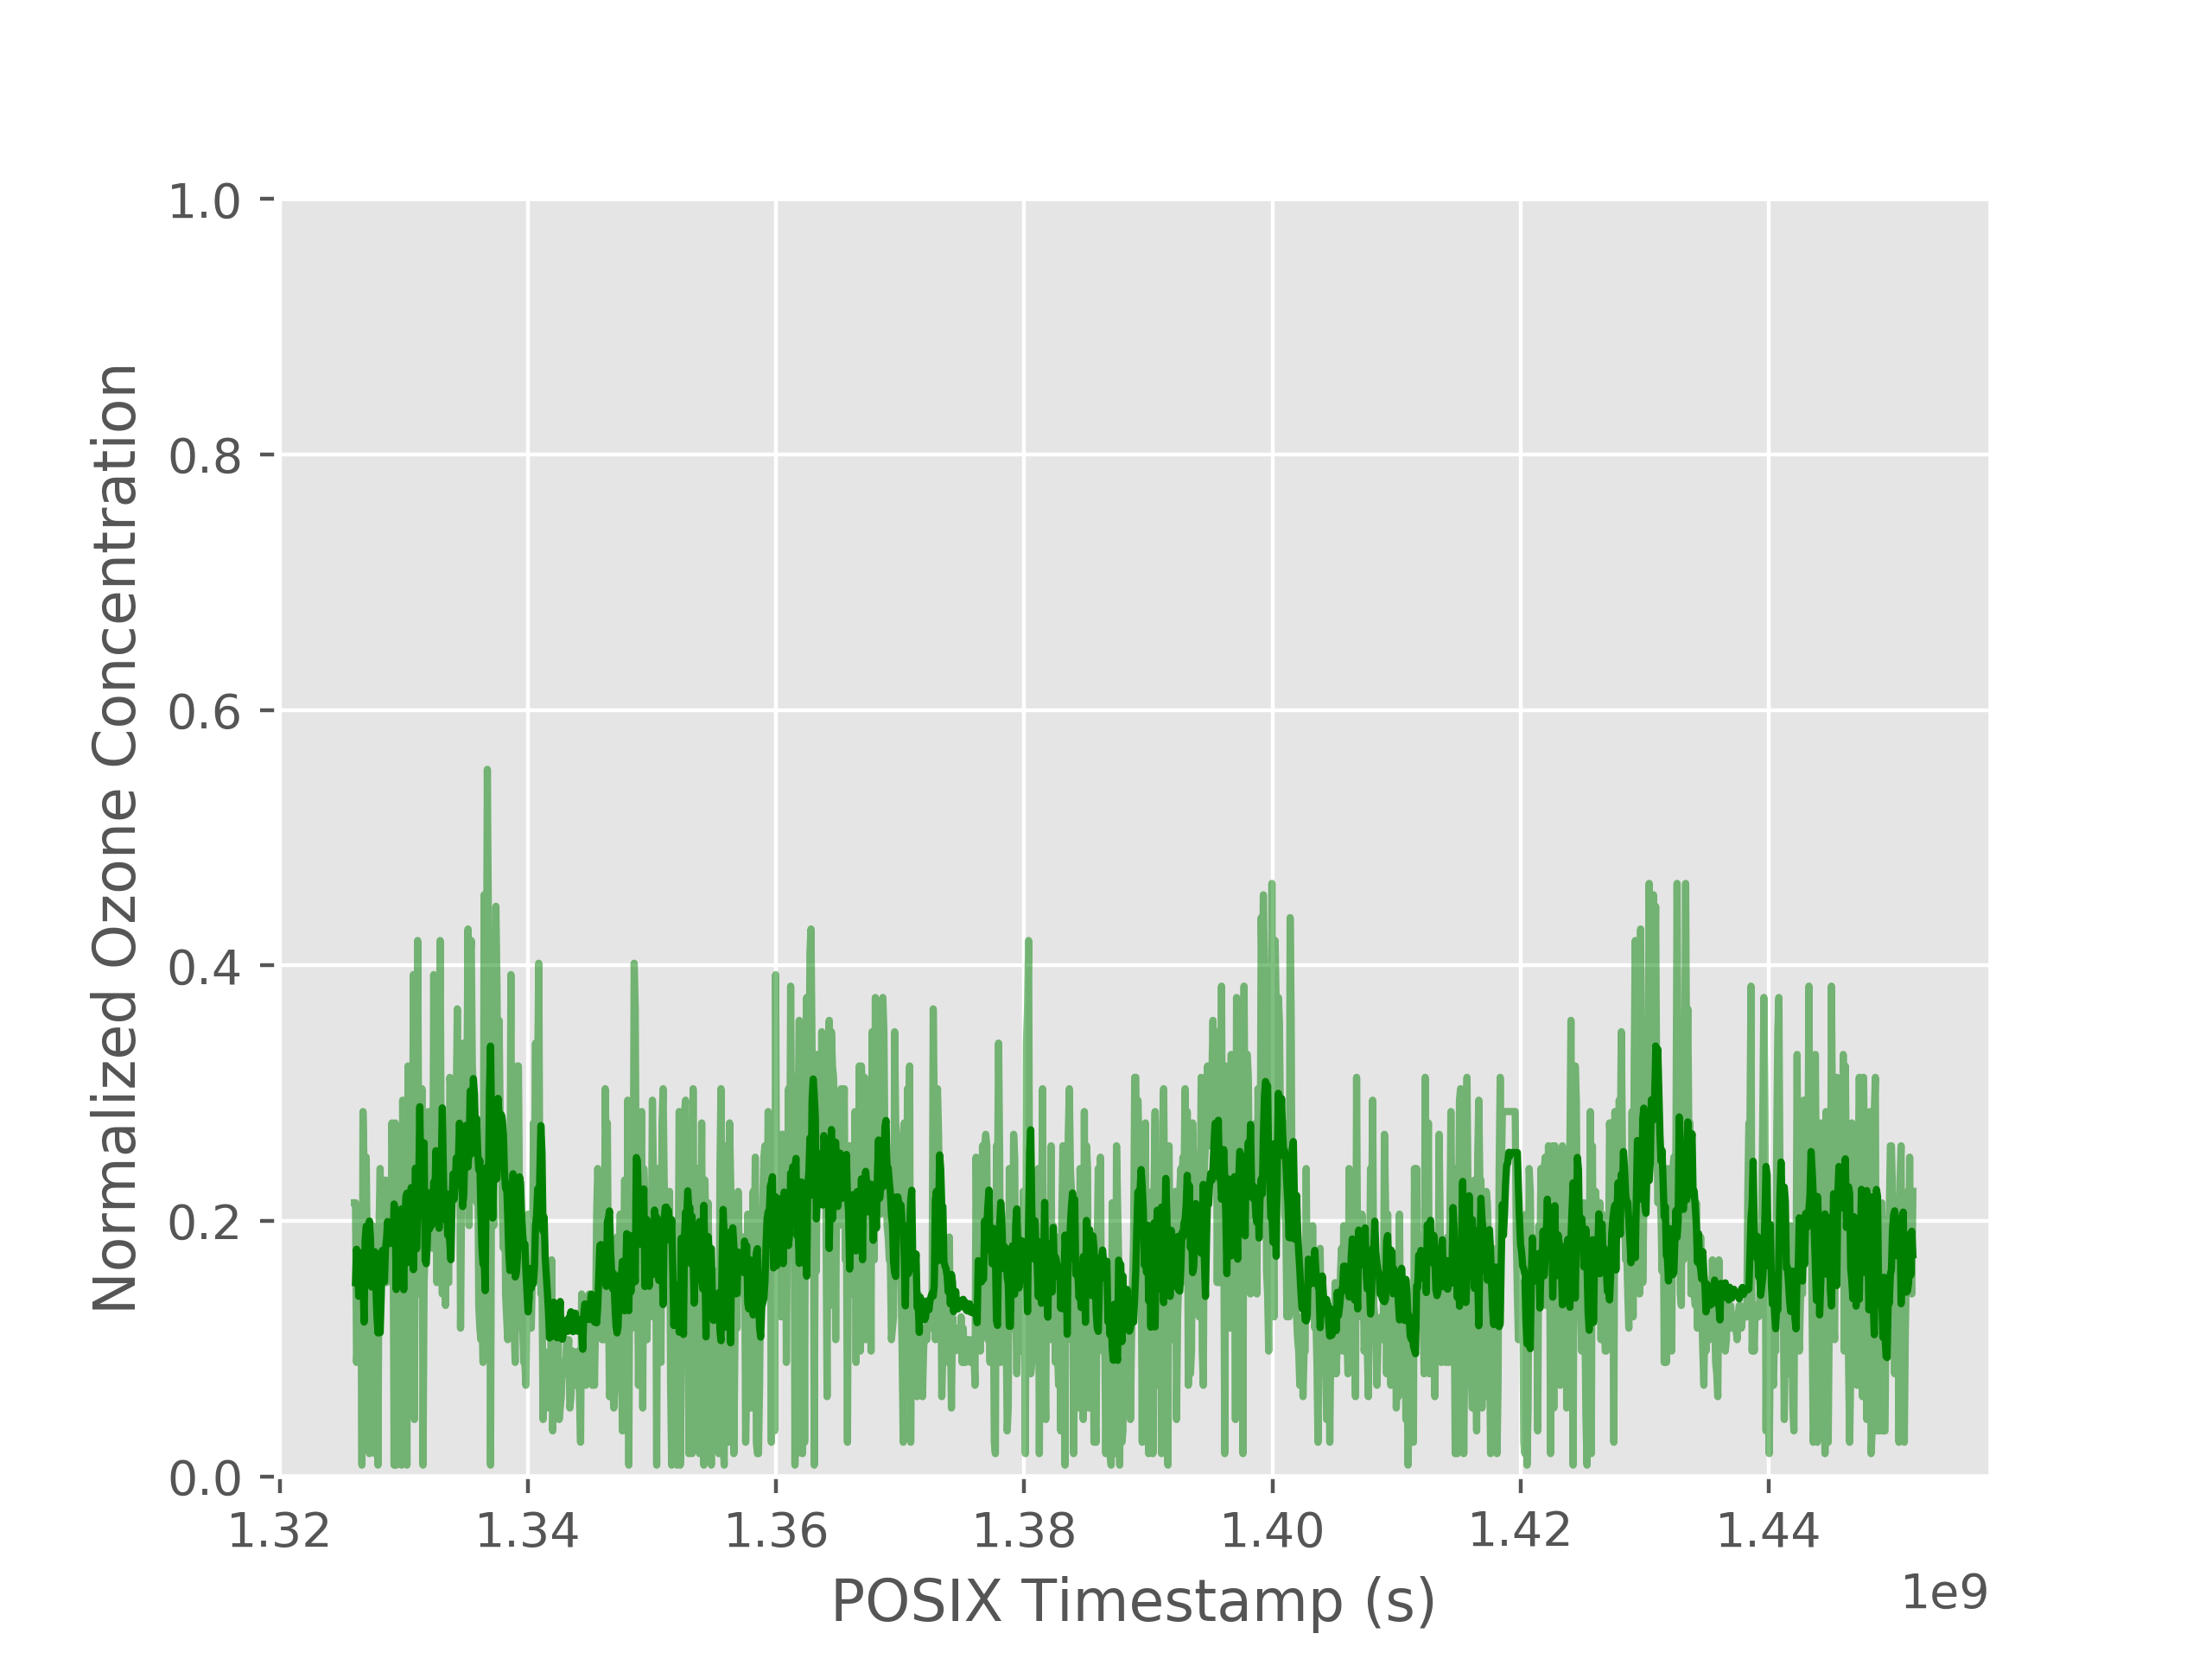
\includegraphics[scale=0.75]{D8_2000_TANH.png}
    \end{center}
    \caption{Graph of actual data values and the best prediction for MLP trained using daily data with a rolling window size of 8.}
\end{figure}

\begin{table}[H]
    \centering
    \begin{tabular}{| c | c | c | c | c |}
        \hline
        \cellcolor{black} & \cellcolor{Gray} 500 & \cellcolor{Gray} 1000 & \cellcolor{Gray} 1500 & \cellcolor{Gray} 2000 \\
        \hline
        \cellcolor{Gray} Identity & 0.1797 & 0.1701 & 0.1839 & 0.1728 \\
        \hline
        \cellcolor{Gray} Logistic & 0.1548 & 0.1662 & 0.1729 & 0.1600 \\
        \hline
        \cellcolor{Gray} Tanh & 0.1696 & 0.1672 & 0.1729 & \cellcolor{green} 0.1862 \\
        \hline
        \cellcolor{Gray} ReLU & 0.1763 & 0.1753 & 0.1575 & 0.1682 \\
        \hline
    \end{tabular}
    \caption{$r^2$ values for the daily time-series predictions of neural networks with different hidden layer activation functions and varying numbers of hidden nodes.}
\end{table}

When attempting to predict one day ahead using data from the previous days, the predictive performance in terms of $r^2$ of the MLP decreases dramatically. It still seems to capture the trends within the data as shown by the "shape" of the curve in figure 2. The increase in the time interval between samples affected the performance of all agents regardless of the parameters selected. Perhaps we can improve performance by adding back data or increasing the size of our rolling window.

\begin{figure}[H]
    \begin{center}
        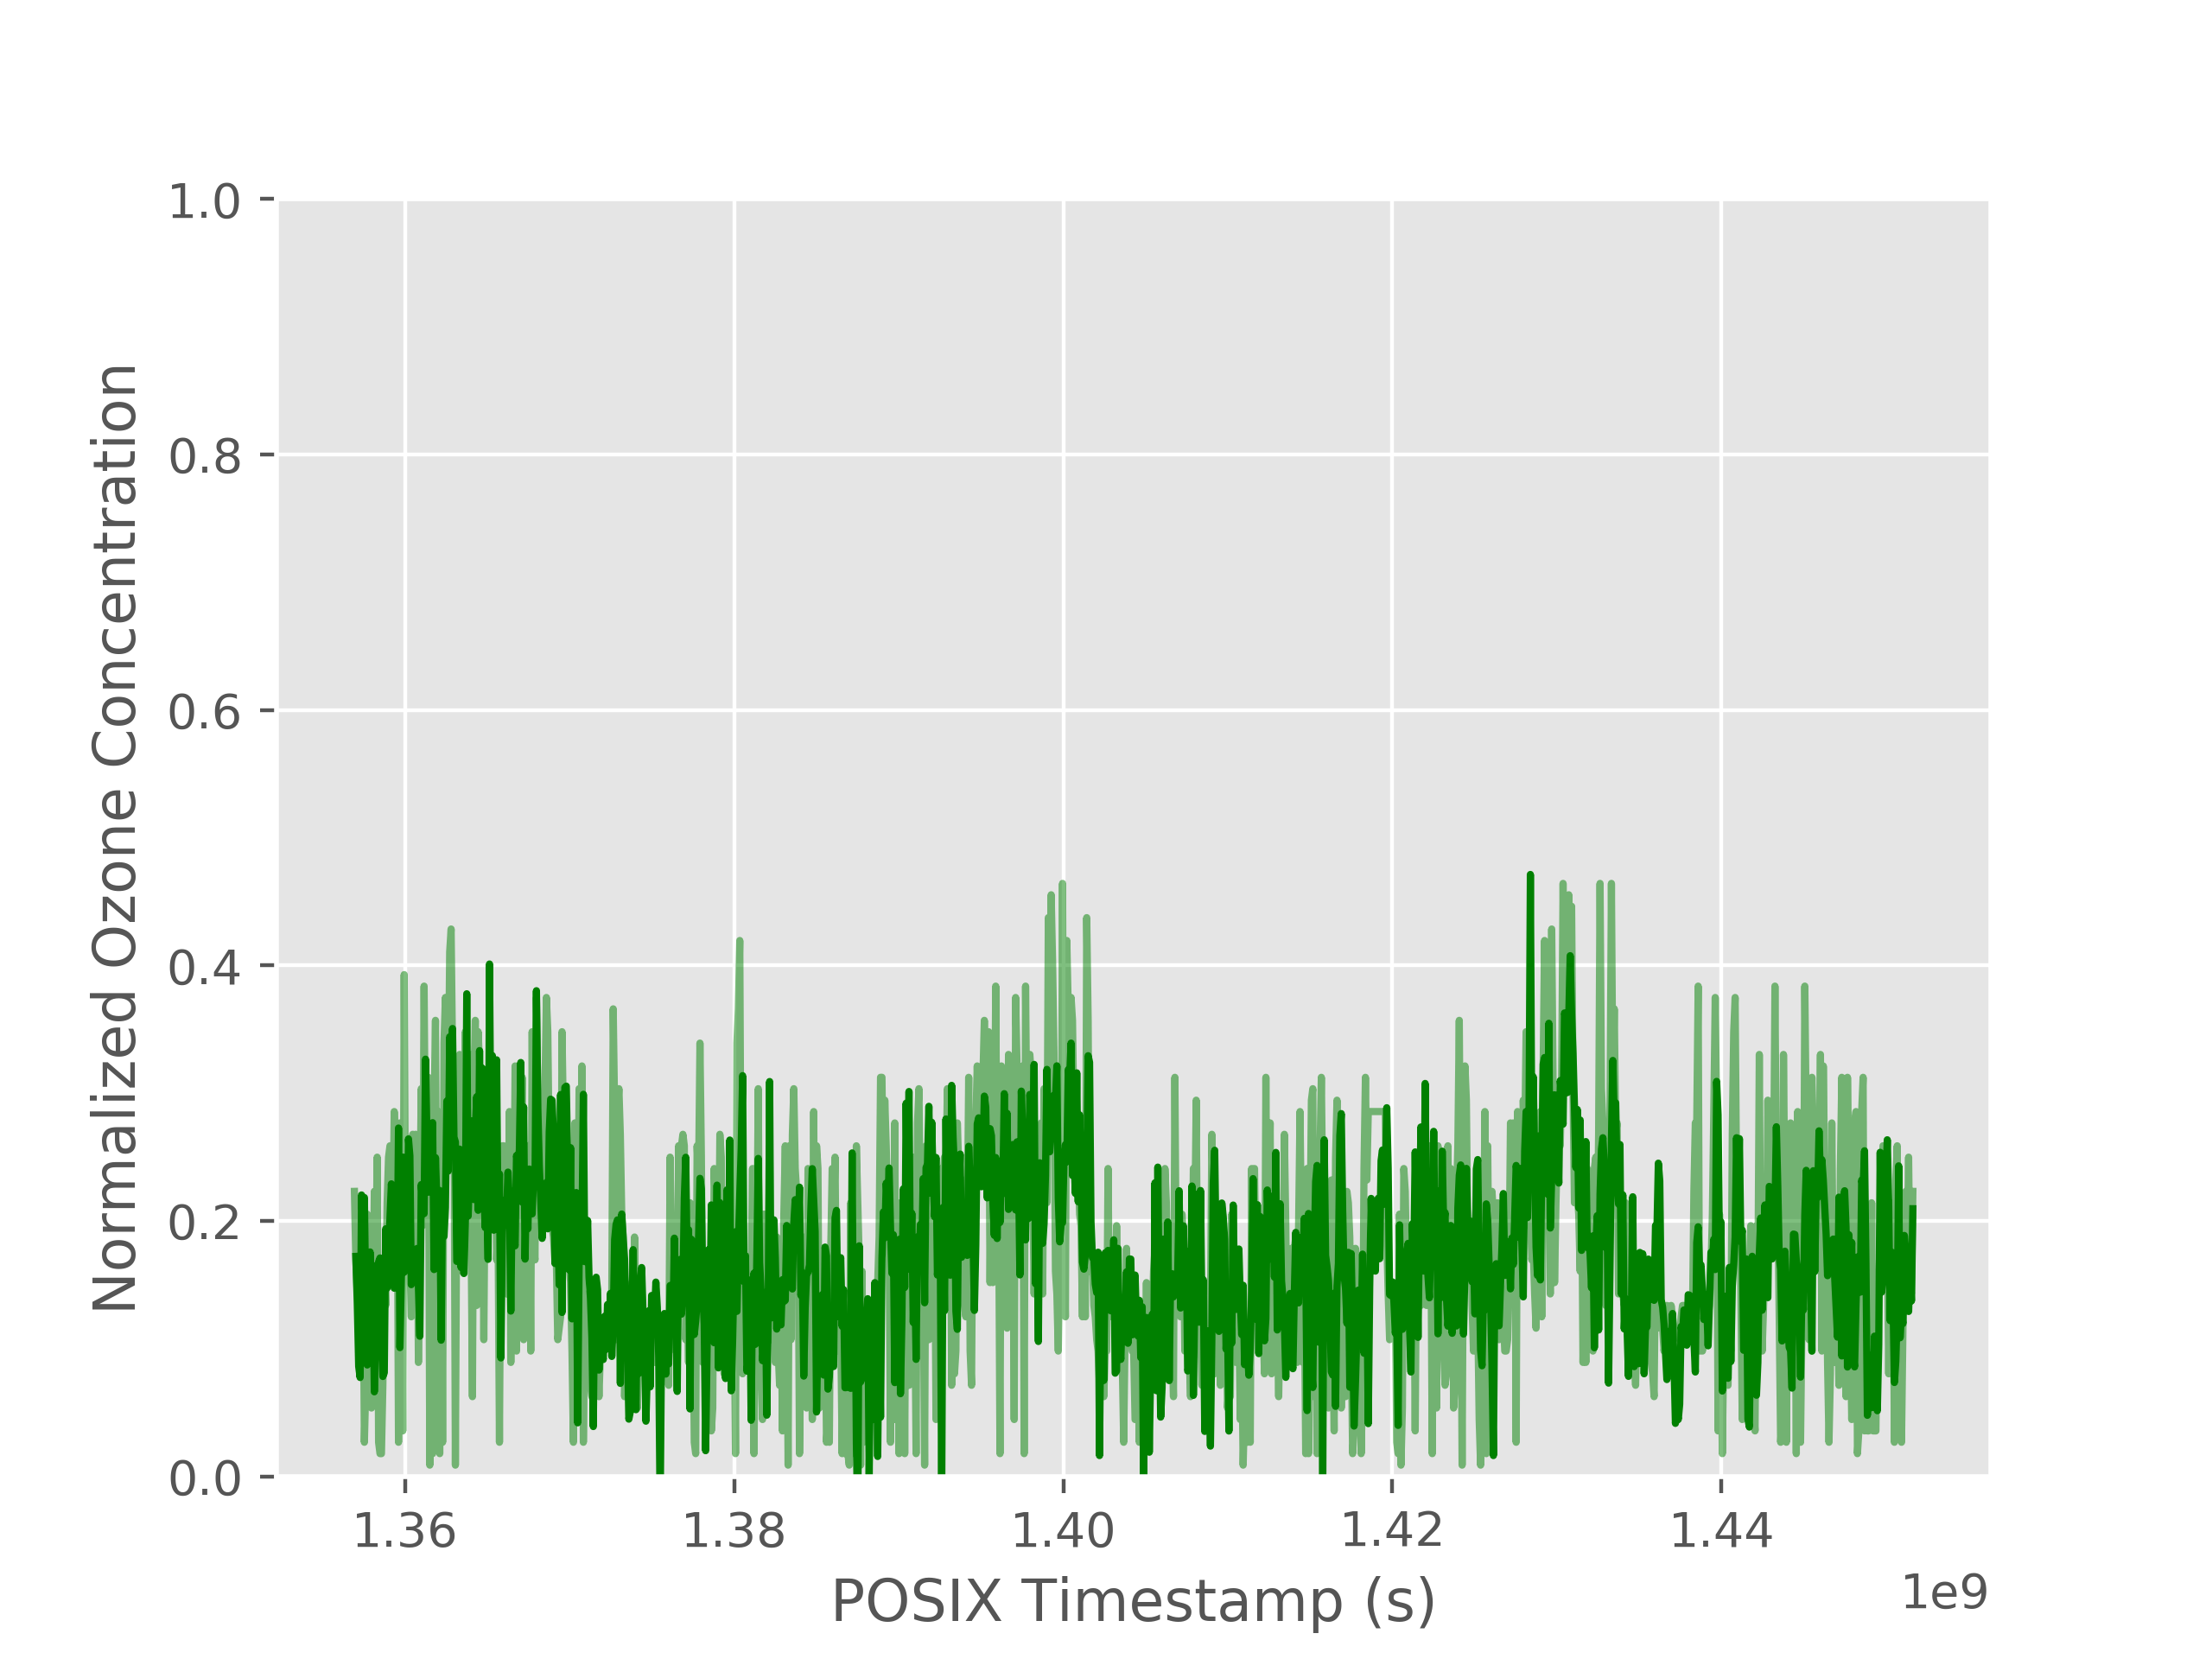
\includegraphics[scale=0.75]{D366_500_TANH.png}
    \end{center}
    \caption{Graph of actual data values and the best prediction for MLP trained using daily data with a rolling window size of 366.}
\end{figure}

\begin{table}[H]
    \centering
    \begin{tabular}{| c | c | c | c | c |}
        \hline
        \cellcolor{black} & \cellcolor{Gray} 500 & \cellcolor{Gray} 1000 & \cellcolor{Gray} 1500 & \cellcolor{Gray} 2000 \\
        \hline
        \cellcolor{Gray} Identity & -0.2563 & -0.1707 & -0.0671 & -0.0082 \\
        \hline
        \cellcolor{Gray} Logistic & 0.1220 & 0.1275 & 0.0926 & 0.1240 \\
        \hline
        \cellcolor{Gray} Tanh & \cellcolor{green} -0.3154 & -0.1511 & -0.1122 & 0.006 \\
        \hline
        \cellcolor{Gray} ReLU & -0.0362 & 0.0577 & 0.0739 & 0.0793 \\
        \hline
    \end{tabular}
    \caption{$r^2$ values for daily time-series predictions of neural networks with different hidden layer activation functions and varying numbers of hidden nodes.}
\end{table}

After we increased the size of the rolling window to 365, the model seems to perform better. Although there are negative $r^2$ values and some that are near zero, the predictions made by the model still closely follow the trend within the data. As previously mentioned, the negative $r^2$ values may indicate that the model needs to incorporate an intercept. The selection of the activation function and number of hidden nodes seems to matter more as the number of features increase.

\section{Discussion}
Ozone concentration prediction is important and the results of experimentation show that it can be done effectively using MLP. Beyond ozone concentration, there are many other important time-series prediction problems like weather, the stock market, and economic growth.

Unfortunately, the effectiveness of the model seems to worsen as the model has to predict further in advance but this may be because time-series prediction is a challenging task. There are many variables at play in the world and there may be many other variables that affect ozone concentration that were not included.

Although this provides the foundation for use of MLP in tackling time-series prediction problems, it is not the end. In the research done on time-series prediction methods, we discovered algorithms such as AutoRegressive Integrated Moving Average (ARIMA) that may be better suited for tackling this problem. Perhaps in the future, a comparison study between the effectiveness of these two methods can be researched to further the idea that MLP is either an effective or ineffective method for solving this class of problems.

\begin{thebibliography}{9}
    \bibitem{oshalimits}
    Ozone Solutions. OSHA and Ozone. \texttt{https://www.ozonesolutions.com/info/osha-and-ozone}

    \bibitem{rollingwindow}
    Srinath Perera. Rolling Window Regression: a Simple Approach for Time Series Next Value Predictions.
    \texttt{https://medium.com/making-sense-of-data/time-series-next-value-prediction} \\
    \texttt{-using-regression-over-a-rolling-window-228f0acae363}

    \bibitem{epanaaqs}
    United States Environmental Protection Agency (EPA). 2015 National Ambient Air Quality Standards (NAAQS) for Ozone. \\
    \texttt{https://www.epa.gov/ground-level-ozone-pollution/2015-national-ambient-air-}
    \texttt{quality-standards-naaqs-ozone}
\end{thebibliography}

\end{document}